
\section{Description: Navigationsframe Lerntool}\label{description}


\subsection{Overview}\label{overview}


Im Lernteil des Mumie-Projektes unterteilt sich das
\textbf{Haupt}browserfenster in folgende Bereiche:

\begin{list_sabina}
        \item \textbf{zentrale Men"uleiste} (f"ur globale Optionen)
        \item \textbf{Navigationsbereich} (f"ur die interaktive Pr"asentation des speziellen Moduls)
        \item \textbf{zentrales Inhaltsfenster} (f"ur den inhaltlichen ``Hauptinput'')
\end{list_sabina}

\begin{figure}[h]
\begin{center}
\ifx\pdfoutput\undefined
  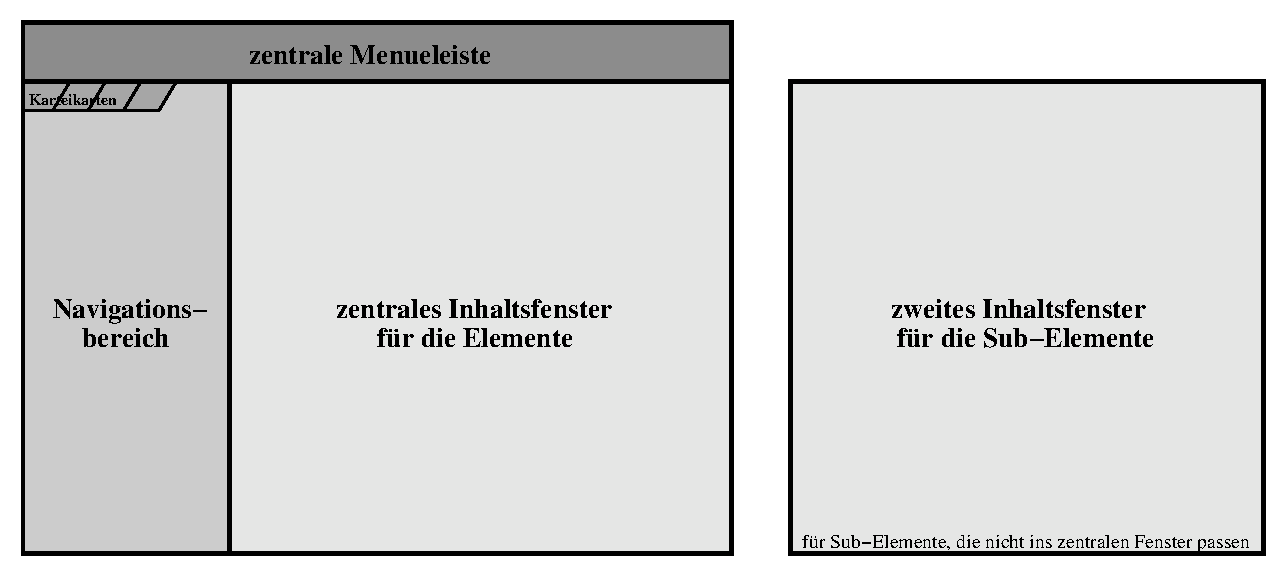
\epsfig{file=Skizzen/gesamtszenario_01.eps, height = 5cm} 
\else
  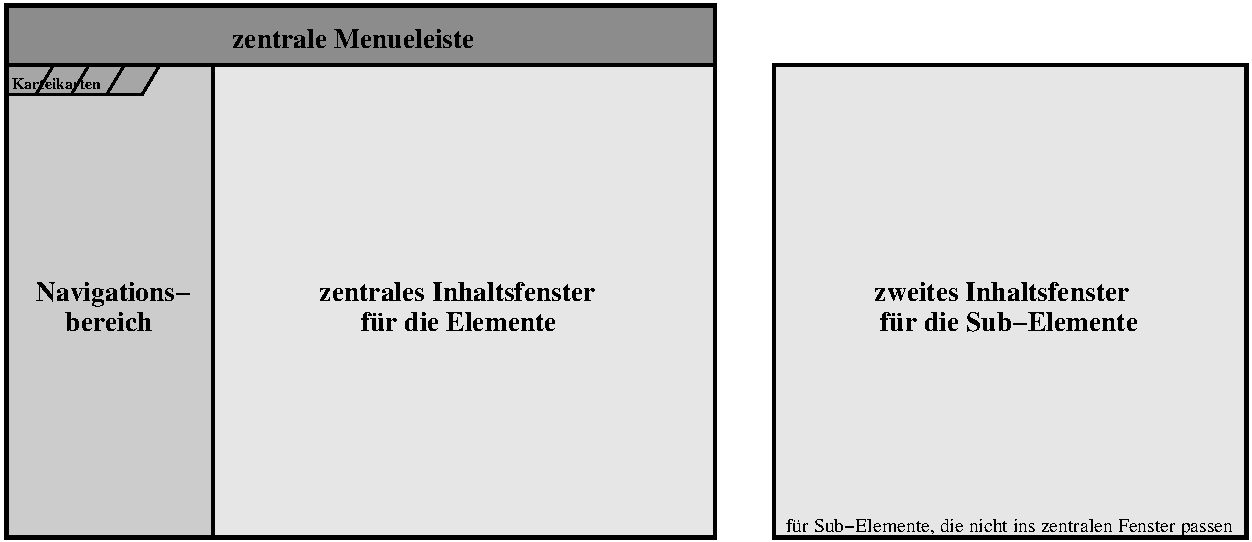
\includegraphics{Skizzen/gesamtszenario_01.pdf}
\fi
\caption{Layout der Hauptansicht im Lerntool}
\end{center}
\end{figure}


Der Navigationsbereich wird auf zwei verschiedene Weisen realisiert:

\begin{list_sabina}
        \item \textbf{Navigationsnetz}: Die Netzdarstellung erlaubt das orientierte
          Navigieren im gew"ahlten Kurs, stellt aber zus"atzlich weitere
          Elemente und alternative Wege dar, die jederzeit mit angew"ahlt
          werden k"onnen. \\
          Die Netzstruktur dient insbesondere der Vermittlung von
          mathematischen Zusammenh"angen: die logischen Abh"angigkeiten der
          Elemente werden durch eine Strichart (``logisches Netz''), 
          der gew"ahlte Kurs durch eine zweite Strichart (``Kurspfad'')
          dargestellt. Forward/Backward-Aktionen beziehen sich stets
          auf den Kurspfad.
        \item \textbf{lineare Navigation:} Die lineare Darstellung (Modell
          etwa wie ein U-Bahn-Plan f"ur eine einzige Linie) stellt nur die
          Elemente des Modules dar, die f"ur den gew"ahlten Kurs vorgesehen
          sind. Alternative Wege und/oder weitere vorhandene Elemente sind in
          dieser Darstellung unsichtbar.\\
	  Die lineare Navigation dient insbesondere dem Ziel, dem 
	  ``Lost-in-Cyberspace''-Effekt entgegenzuwirken.
\end{list_sabina}


Ausgangspunkt f"ur die Darstellung ist zun"achst das Navigationsnetz (hier
wird auf Alternativen erst aufmerksam gemacht, deren Existenz andernfalls
nicht sichtbar ist). Zwischen den beiden Navigationsformen kann zu jeden
Zeitpunkt geswitched werden (Karteikartensytem am oberen Rand des
Navigationsbereiches).


Im folgenden werden beide Navigationsbereiche im Detail beschrieben.

\subsection{Karteikartensystem}

\subsubsection{General Remarks}

Zwischen den verschiedenen Ansichten (Navigationsnetz und Lineare
Navigation) wird durch ein Karteikartensystem hin- und hergeschaltet,
welches dar"uber hinaus weitere Karten verwaltet:

\begin{list_sabina}
        \item \textbf{1. Navigationsnetz:}
        definiert in Kap. \ref{navigationsnetz}
        \item \textbf{2. Lineare Navigation:}
	definiert in Kap. \ref{lineare_navigation}
         \item \textbf{3. Summary:}
        Zusammenfassung eines Modules \\
	(Stichwort: Vorschl"age nach V. En"s, to be specified)
        \item \textbf{4. Notes:}
        eigene Bemerkungen und Statusanzeigen, angelegt vom User \\
	(Stichwort: nach Linguistikprojekt, gesehen in K"oln, to be specified)
\end{list_sabina}

Die Karten werden durch Icons gekennzeichnet.\\
Aktivieren einer Karteikarte markiert deren Auswahl durch farbliche
"Anderung, highlighting etc.

Layouttechnisch muss das Auftreten von mindestens zwei weiteren
Karteikarten eingeplant werden (insbesondere auch im Hinblick auf die
"ubrigen Tools).

\begin{figure}[h]
\begin{center}
\ifx\pdfoutput\undefined
   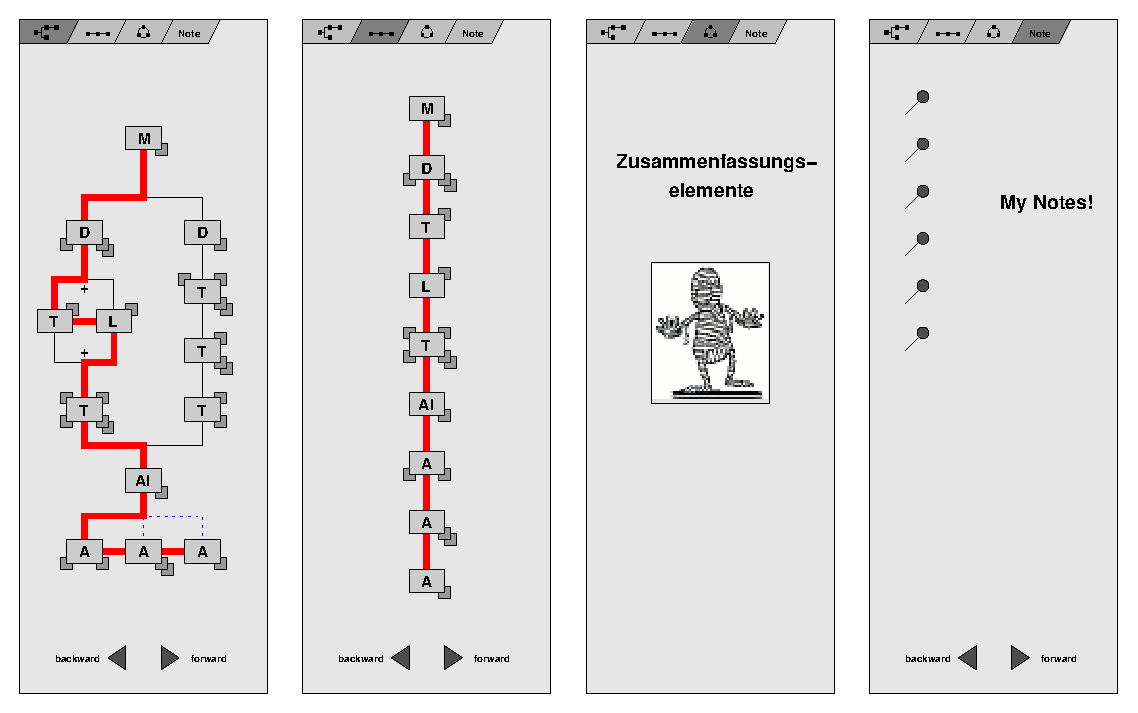
\epsfig{file=Skizzen/all_cards.eps, height=80mm} 
\else
  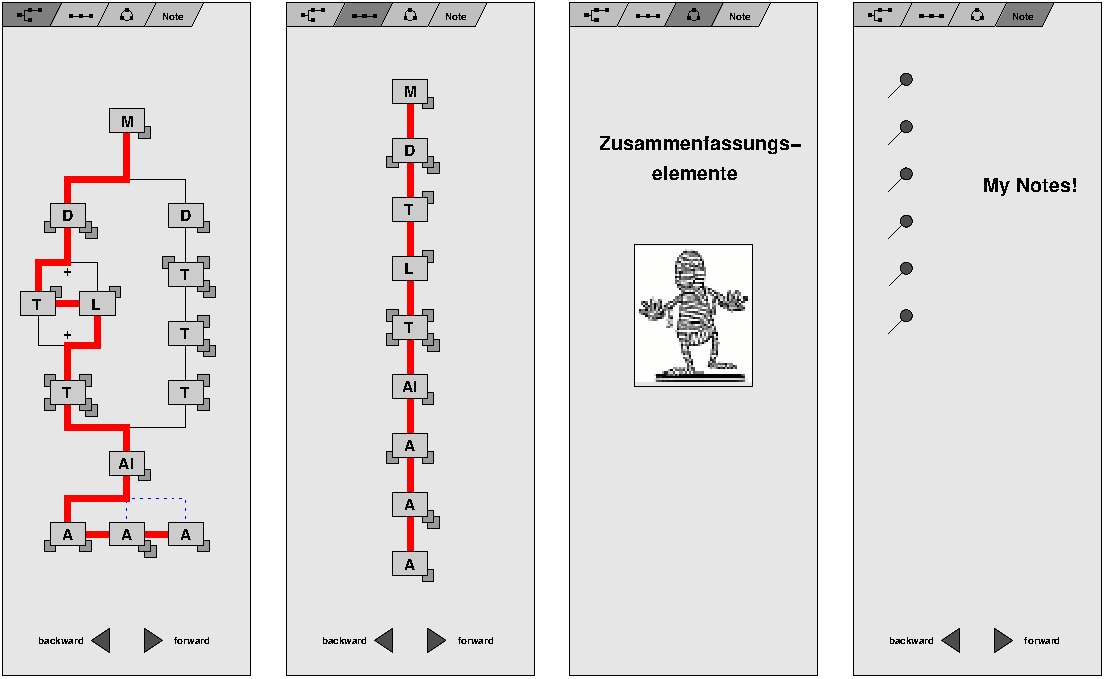
\includegraphics{Skizzen/all_cards.pdf}
\fi
\caption{Umschalten durch Karteikarten}
\end{center}
\end{figure}


\clearpage

\subsection{Navigationsnetz}\label{navigationsnetz}


\subsubsection{General Remarks}

In der Navigationliste wird zun"achst das logische Netz des Moduls
abgebildet, dar"uber wird der ``Kurspfad'' dargestellt, der den roten,
zeitlich orientierten Faden durch den gew"ahlten bzw. durch den in
Abh"angigkeit vom Benutzerprofil empfohlenen Kurs repr"asentiert.\\
Die abgebildete Pfadstruktur ist bewu"st \emph{nicht-linear}: Der Studierende
soll neben den reinen Inhalten auch deren Zusammenh"ange und Abh"angigkeit
visuell erleben k"onnen.


\subsubsection{Design und Anordnungsregeln der (Sub-)Elemente}

\paragraph{Design der (Sub-)Elemente}\mbox{ }\label{netz:design_sub_und_elemente}\\[-2ex]

Die Elemente sollen zun"achst durch farbige, leicht dreidimensional
angedeutete, anclickbare K"astchen dargestellt werden (Vorschlag f"ur
1. Entwurf), in denen sich eine Abk"urzung und/oder ein Icon befindet,
das die Art des Elements angibt: T f"ur Theorem, D f"ur Definition,...
(serifenloser Font).\\
Die Subelemente werden in kleineren K"astchen leicht hinter die Elemente
geh"angt, in einheitlicher Farbe und aus Platzgr"unden \textit{ohne} weitere
Unterscheidungsmarkierung. Dabei gelten die Anordnungsregeln aus
Kap. \ref{netz:anordnungsregeln}.\\

Die verf"ugbaren Elemente:
\begin{center}
\begin{tabular}{|l|l|l|}
\hline
Motivation              & (M)   & eigene Farbe          \\
\hline
\hline
Definition              & (D)   & eigene Farbe          \\
\hline
Theorem                 & (T)   & eigene Farbe          \\
\hline
Lemma (Hilfssatz)       & (L)   & Farbe wie Theorem     \\
\hline
Algorithmus             & (Al)  & eigene Farbe          \\
\hline
\hline
Anwendung               & (A)   & eigene Farbe          \\
\hline
\end{tabular}
\end{center}

Die verf"ugbaren Subelemente:
\begin{center}
\begin{tabular}{|l|l|l|l|}
\hline
Herleitung                                      & Her.  & onecolor (grau?)      & oben links\\
\hline
Beweis                                          & Bew.  & onecolor (grau?)      & oben rechts\\
\hline
Motivation \footnotesize{(zum Hauptelement)}    & Mot.  & onecolor (grau?)      & unten links\\
\hline
Bemerkung                                       & Bem.  & onecolor (grau?)      & unten links\\
\hline
Historisches                                    & Hist. & onecolor (grau?)      & unten links\\
\hline
Visualisierung                                  & Vis.  & onecolor (grau?)      & unten rechts\\
\hline
Beispiel                                        & Bsp.  & onecolor (grau?)      & unten rechts\\
\hline
Tabelle                                         & Tab.  & onecolor (grau?)      & unten rechts\\
\hline
\end{tabular}
\end{center}

\clearpage

\paragraph{An- und Zuordnungsregel der (Sub-)Elemente}\label{netz:anordnungsregeln}\mbox{ }\\[-2ex]


Es gelten die folgenden Anordnungs- und Positionierungsregeln f"ur das
Anh"angen der Subelemente an ihre Elemente (liegen zu einem Element
nicht alle prinzipiell verf"ugbaren Subelemente vor, so r"ucken die
"au"seren nach innen nach):

\fbox{\begin{minipage}[t][61mm]{66mm}
\textbf{Motivation:}
\begin{center}
\ifx\pdfoutput\undefined
   
\epsfig{file=Skizzen/elemente_an_mot_mini.eps}
\else
  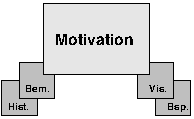
\includegraphics{Skizzen/elemente_an_mot_mini.pdf}
\fi
\end{center}
\vfill
verf"ugb. Subelemente:\\[-4ex]
\begin{flushright}
Bem., Historisches\\
Visualisierung, Bsp.
\end{flushright}
\end{minipage}}
\hfill
\fbox{\begin{minipage}[t][61mm]{66mm}
\textbf{Definition:}
\begin{center}
\ifx\pdfoutput\undefined
   
\epsfig{file=Skizzen/elemente_an_def_mini.eps}
\else
  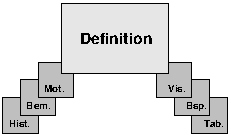
\includegraphics{Skizzen/elemente_an_def_mini.pdf}
\fi
\end{center}
\vfill
verf"ugb. Subelemente:\\[-4ex]
\begin{flushright}
Mot. zu ..., Bem., Historisches\\
Visualisierung, Bsp., Tabelle
\end{flushright}
\end{minipage}}

\vspace{2mm}

\fbox{\begin{minipage}[t][61mm]{66mm}
\textbf{Theorem:}
\begin{center}
\ifx\pdfoutput\undefined
   
\epsfig{file=Skizzen/elemente_an_theorem_mini.eps}
\else
  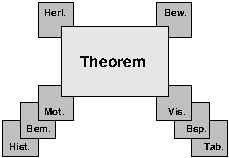
\includegraphics{Skizzen/elemente_an_theorem_mini.pdf}
\fi
\end{center}
\vfill
verf"ugb. Subelemente:\\[-5ex]
\begin{flushright}
Herleitung\\
Beweis\\
Mot. zu ..., Bem., Historisches\\
Visualisierung, Bsp., Tabelle
\end{flushright}
\end{minipage}}
\hfill
\fbox{\begin{minipage}[t][61mm]{66mm}
\textbf{Lemma:}
\begin{center}
\ifx\pdfoutput\undefined
   
\epsfig{file=Skizzen/elemente_an_lemma_mini.eps}
\else
  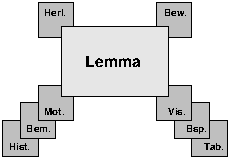
\includegraphics{Skizzen/elemente_an_lemma_mini.pdf}
\fi
\end{center}
\vfill
verf"ugb. Subelemente:\\[-5ex]
\begin{flushright}
Herleitung\\
Beweis\\
Mot. zu ..., Bem., Historisches\\
Visualisierung, Bsp., Tabelle
\end{flushright}
\end{minipage}}

\vspace{2mm}

\fbox{\begin{minipage}[t][61mm]{66mm}
\textbf{Algorithmus:}
\begin{center}
\ifx\pdfoutput\undefined
   
\epsfig{file=Skizzen/elemente_an_algo_mini.eps}
\else
  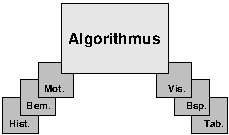
\includegraphics{Skizzen/elemente_an_algo_mini.pdf}
\fi
\end{center}
\vfill
verf"ugb. Subelemente:\\[-4ex]
\begin{flushright}
Mot. zu ..., Bem., Historisches\\
Visualisierung, Bsp., Tabelle
\end{flushright}
\end{minipage}}
\hfill
\fbox{\begin{minipage}[t][61mm]{66mm}
\textbf{Anwendung:}
\begin{center}
\ifx\pdfoutput\undefined
   
\epsfig{file=Skizzen/elemente_an_anwend_mini.eps}
\else
  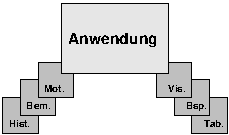
\includegraphics{Skizzen/elemente_an_anwend_mini.pdf}
\fi
\end{center}
\vfill
verf"ugb. Subelemente:\\[-4ex]
\begin{flushright}
Mot. zu ..., Bem., Historisches\\
Visualisierung, Bsp., Tabelle
\end{flushright}
\end{minipage}}

\clearpage

\subsubsection{Verbindungslinien}\label{}

Es existieren zwei Arten von Verbindungslinien: 

\begin{list_sabina}
        \item \textbf{logisches Netz}
        \item \textbf{Kurspfad} 
\end{list_sabina}


\paragraph{Das logische Netz}\mbox{ }\\[-2ex]

Die logischen Abh"angigkeiten werden durch (d"unne, schwarze?) Linien
zwischen den Elementen abgebildet, soweit sie im
mathematisch-fachlichen Sinn bestehen.

Das bedeutet insbesondere: \\
Motivationen werden stets an erster Position gezeichnet, aber nicht
durch Linien mit dem Anschlusselement verbunden.\\
Anwendungen werden in letzter Position gezeichnet und ebenfalls nicht
verbunden.\\
Definitionen, Theoreme, Lemmata und Algorithmen bilden den zentralen
mittleren Block und m"ussen stets untereinander verbunden werden. \\
An jeder Gabelung wird zwischen ``und''- und ``oder''-Verbindung
unterschieden (``+''-Icon f"ur ``und'', ``oder'' ohne Icon).

\begin{figure}[h]
\begin{center}
\ifx\pdfoutput\undefined
   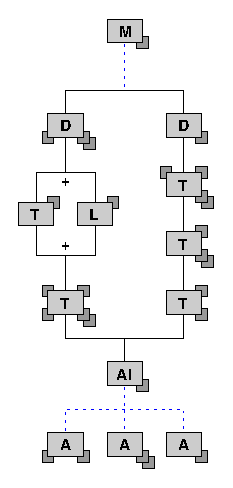
\epsfig{file=Skizzen/navi_drittel.eps}
\else
  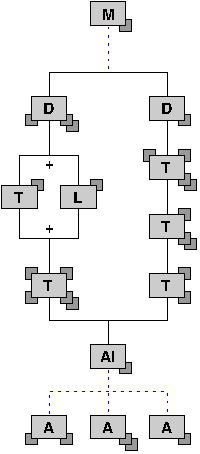
\includegraphics{Skizzen/navi_drittel.pdf}
\fi
\caption{Logisches Netz, logische Verbindungen, ohne Kurspfad}
\end{center}
\end{figure}

\clearpage

\paragraph{Der Kurspfad}\mbox{ }\\[-2ex]

"Uber das Netz der logischen Abh"angigkeiten wird ein ``roter Faden''
gelegt, der der linearen Anordnung der Inhalte in einem Kurs
entspricht.

Das bedeutet insbesondere: \\
``Oder''-Verzweigungen f"uhren auf i.f. unterschiedliche Kurse; 
jede auftretende ``Oder''-Verzweigung f"uhrt auf ein weiteres Bild, 
das generiert werden muss.\\
Bei ``Und''-Verbindungen m"ussen (in einer definierten Reihenfolge) beide
Teile durchlaufen werden, der rote Faden liegt daher nicht mehr auf
den logischen Linien (siehe Abb. \ref{kurs_mit_rotem_faden} links).

\begin{figure}[h]
\begin{center}
\ifx\pdfoutput\undefined
   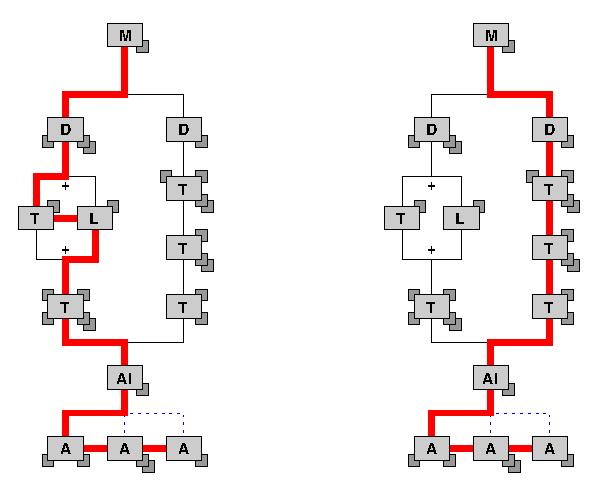
\epsfig{file=Skizzen/navi_drittel_kurs.eps}
\else
  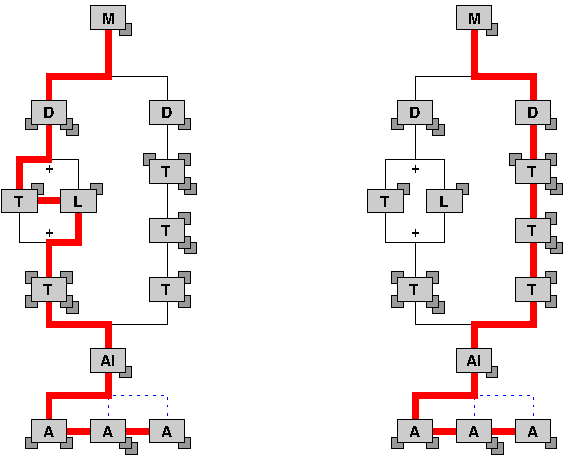
\includegraphics{Skizzen/navi_drittel_kurs.pdf}
\fi
\caption{M"ogliche Kurspfade mit rotem Faden}\label{kurs_mit_rotem_faden}
\end{center}
\end{figure}

Um den aktiven Kurspfad zus"atzlich hervorzuheben, sollte der nicht
zum Kurspfad geh"orende Teil leicht in den Hintergrund gelegt werden,
ohne aber seine Funktionalit"at grunds"atzlich zu verlieren.

\clearpage

\subsubsection{Mouse-Aktionen}\label{netz:mouse_actions}

Mouse-Aktionen k"onnen weitere "Ubersichtsm"oglichkeiten schaffen:

\begin{list_sabina}
        \item \textbf{Mouse-over}\\
        Zoom-Effekt, Element mit seinen Subelementen erscheint
        vergr"o"sert, Subelemente werden in dieser Darstellung
	unterscheidbar durch Beschriftung

\begin{figure}[h]
\begin{center}
\ifx\pdfoutput\undefined
   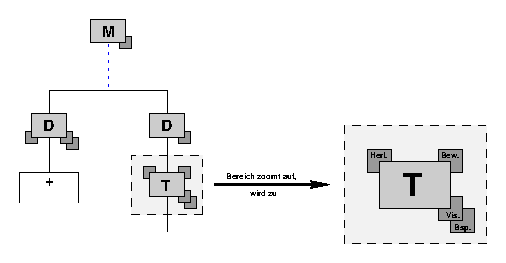
\epsfig{file=Skizzen/zoom_element.eps} 
\else
  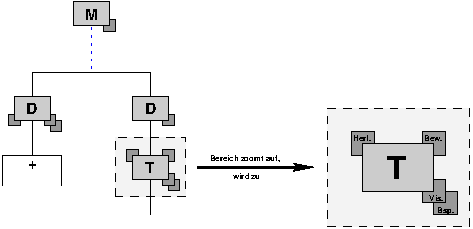
\includegraphics{Skizzen/zoom_element.pdf}
\fi
\caption{Detailansicht bei Mouse-Over}
\end{center}
\end{figure}

        \item \textbf{Mouse-out}\\
        Zoom-Effekt verschwindet wieder
        \item \textbf{Left-Mouse-Click}\\
        Inhalt erscheint im zentralen Inhaltsfenster
        \item \textbf{Middle-Mouse-Click}\\
        Inhalt erscheint, aber in Extrafenster 
        \item \textbf{Right-Mouse-Click}\\
        Menue mit Optionen erscheint (Standard bei Browsern)
\end{list_sabina}

\clearpage


\subsubsection{Forward/Backward-Button}\label{}

Der ``Forward/Backward-Button'' erm"oglicht die Bewegung entlang des
roten Fadens in einfacher Weise.  Die M"oglichkeit, K"astchen
alternativ \textit{direkt} anzuclicken, wird dadurch nicht ber"uhrt.

Der ``Forward/Backward-Button'' ist aktiv, solange der User sich
innerhalb seines Kurspfades befindet, anderenfalls ist er inaktiv
(ausgegraut).

Layout-Skizze:

\begin{figure}[h]
\begin{center}
\ifx\pdfoutput\undefined
   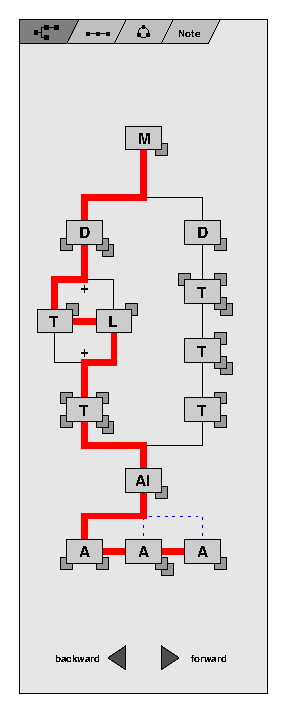
\epsfig{file=Skizzen/navinetz_komplett.eps} 
\else
  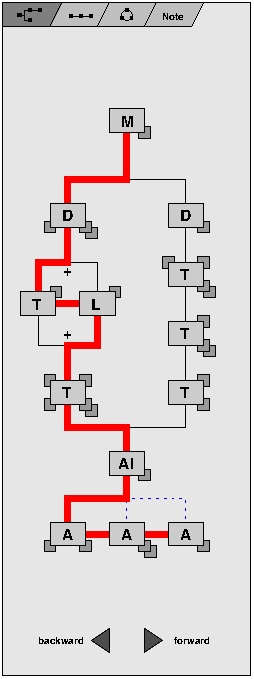
\includegraphics{Skizzen/navinetz_komplett.pdf}
\fi
\caption{Navigationsnetz mit ``Forward/Backward-Button''}
\end{center}
\end{figure}


\clearpage

\subsection{Lineare Navigation}\label{lineare_navigation}

\subsubsection{General Remarks}

In der Navigationsleiste wird eine Voll-Linearisierung des gew"ahlten
Kurses abgebildet.

\subsubsection{Design und Anordnungsregeln der (Sub-)Elemente}

Farb- und Formgebung sowie Anordnungsregeln werden identisch zu der
beim Navigationsnetz gew"ahlten verwendet
(s. S. \pageref{netz:design_sub_und_elemente},
\pageref{netz:anordnungsregeln}).

\subsubsection{Verbindungslinien}\label{}

Es exisiert genau eine Verbindungslinie:

\begin{figure}[h]
\begin{center}
\ifx\pdfoutput\undefined
   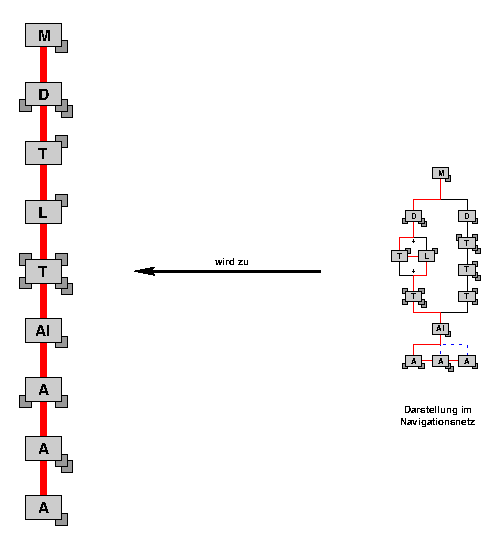
\epsfig{file=Skizzen/lineare_navi_wandel.eps} 
\else
  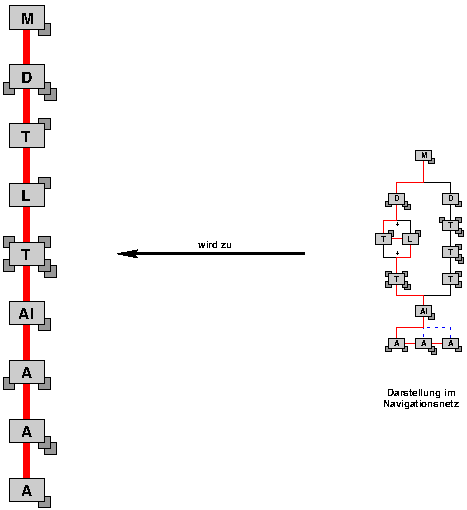
\includegraphics{Skizzen/lineare_navi_wandel.pdf}
\fi
\caption{Verbindungslinien bei der linearen Navigation}
\end{center}
\end{figure}

\clearpage

\subsubsection{Mouse-Aktionen}

Mouse-Aktionen werden identisch zu den beim Navigationsnetz gew"ahlten
verwendet (s. S. \pageref{netz:mouse_actions}).

\subsubsection{Forward/Backward-Button}\label{}

Der ``Forward/Backward-Button'' erm"oglicht die Bewegung entlang des
roten Fadens in einfacher Weise.  Die M"oglichkeit, K"astchen
alternativ \textit{direkt} anzuclicken, wird dadurch nicht ber"uhrt.

Der ``Forward/Backward-Button'' ist stets aktiv.

Layout-Skizze:

\begin{figure}[h]
\begin{center}
\ifx\pdfoutput\undefined
   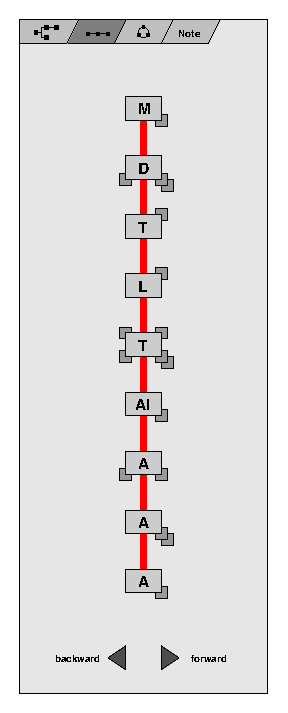
\epsfig{file=Skizzen/linear_komplett.eps} 
\else
  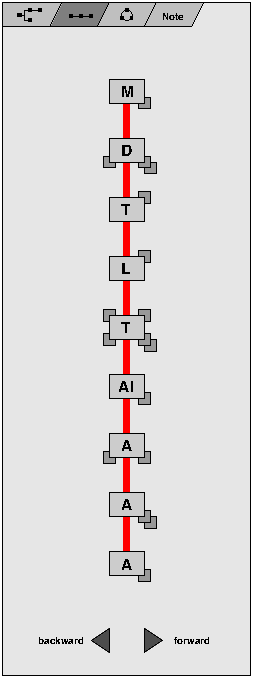
\includegraphics{Skizzen/linear_komplett.pdf}
\fi
\caption{Lineare Navigation mit ``Forward/Backward-Button''}
\end{center}
\end{figure}

\clearpage

\subsection{Summary}\label{Summanry}

t.b.c. 	(Stichwort: Vorschl"age nach V. En"s, to be specified)

\clearpage

\subsection{MyNotes}\label{my_notes}

t.b.c.	(Stichwort: nach Linguistikprojekt, gesehen in K"oln, to be specified)

\clearpage

\subsection{Additional -- Erg"anzungen, Bemerkungen etc.}\label{additional}

In diesem Kapitel werden Erg"anzungen und Anmerkungen zur
Navigationsframe im Lerntool kontinuierlich fortgeschrieben:

\begin{list_sabina}
        \item \textbf{Gr"o"se -- Skalierung}: 
	Navigationsnetz und lineare Navigation m"ussen das vorhandene
	Navigationsfenster in optimaler Weise ausnutzen (flexibler
	Algorithmus; konstante K"astchengr"o"se, aber flexible
	Linienanpassung).
	Scrollbars sind unter allen Umst"anden zu vermeiden.\\
	F"ur sp"atere Versionen (h"ohere Aufl"osung $\Rightarrow$
	gr"o"seres Fenster) m"ussen die Graphiken einfach angepasst
	werden k"onnen
	(Gr"o"se des Navigationsframes als Variablen "ubergeben).
        \item \textbf{Und- und Oder-Verbindungen}: 
	Es ist zu kl"aren, wie ``und-Verbindungen tats"achlich gezeichnet
	werden sollen: mit ``+''-Icon oben und unten oder nur unten...
	In den Skizzen wurde zur Klarheit oben und unten das ``+''-Icon 
	gesetzt.
\end{list_sabina}




